\input{D:/Physics/Program/Book-begin.tex}
\usepackage{ctex}
\usepackage{multirow}  % 允许单元格合并
\usepackage{booktabs}  % 提供更美观的表格线

\title{\textbf{Documentation for GEONU Software}}
\author{Shuai Ouyang\thanks{\parbox[t]{4.5cm}{%
			\texttt{shuaiouyang@mail.sdu.edu.cn} \\ 
			\texttt{Shuai.Ouyang@snolab.ca}}}}
\date{2025.03.21}

\begin{document}
	\pdfbookmark{Book Cover}{title} 	%创建封面pdf标签;第一个{}参数是pdf标签的名字,第二个{}参数用于hyperlink,
	\maketitle							%显示封面
	\thispagestyle{empty}				%封面取消页码
	\frontmatter						%页码使用罗马字母
	\cleardoublepage				 	%消除一张空白页,为了在pdf中实现目录的跳转
	\pdfbookmark{\contentsname}{toc} 	%创建目录pdf标签
	\tableofcontents				  	%生成目录
	\mainmatter							%页码使用拉丁数
	\chapter{介绍}
		\section{什么是地球中微子}
			简单来说,Geonu指的是来自地球内部的中微子。这个课题的研究来自于地质学,早先地质学家通过地震波研究清楚了地球的内部结构,对地球内部的物理性质了解的十分清楚,但对化学性质却知之甚少。地球的化学性质对于地球的演化非常重要,例如地球表面的大陆板块运动、地幔的物质循环就十分依赖地球内部化学性质。目前也有不少能够描述地球内部化学性质的理论,但是人类的地下活动仅仅$12$ km,并没有多少关于地幔的直接测量数据,所以需要实验来辨别哪些理论是正确的,哪些理论是错误的。\par
			推动地球内部运动的能量来源一部分来自于元素的衰变,这些元素统一被称作HPE。地质学家注意到HPE衰变,例如${}^{235}U, {}^{238}U, {}^{232}Th, {}^{40}K$,在产生热量的同时会释放中微子\cite{fiorentini2007geo} (Eq.\ref{Decay:U235}-\ref{Decay:K40_2});由于中微子只参与弱相互作用,所以它可以很轻易地将地球内部的信息传递出来,所以地球中微子成为了人类认识地球内部化学性质的一个重要手段。
				\begin{align}
					&{}^{235}U \longrightarrow {}^{207}Pb + {}^{4}He + 4e^- + 4\overline{\nu}_e + 0.283 \text{ MeV},
					\label{Decay:U235}\\
					&{}^{238}U \longrightarrow {}^{206}Pb + 8\alpha + 6e^- + 6\overline{\nu}_e + 51.7 \text{ MeV},
					\label{Decay:U238}\\
					&{}^{232}Th \longrightarrow {}^{208}Pb + 6\alpha + 4e^- + 4\overline{\nu}_e + 42.7 \text{ MeV},
					\label{Decay:Th232}\\
					&{}^{40}K \overunderset{\longrightarrow}{(89.3\%)} {}^{40}Ca + e^- + \overline{\nu}_e + 1.31 \text{ MeV},
					\label{Decay:K40_1}\\
					&{}^{40}K \overunderset{\longrightarrow}{(10.7\%)} {}^{40}Ar + \nu_e + 1.505 \text{ MeV}.
					\label{Decay:K40_2}
				\end{align}
			目前探测地球中微子的方式是通过IBD反应:
				\begin{equation}
					\overline{\nu}_e + p \longrightarrow n + e^+,
				\end{equation}
			正电子迅速与电子湮灭,在实验上产生promt信号;中子之后随机游走,并且在游走的过程中能量逐渐降低,最终被质子俘获从而在实验上产生delayed信号。由于这个反应的阈值为$1.806$ MeV,目前人类只能看到来自${}^{238}U$和${}^{232}Th$衰变的地球中微子(图\ref{Fig:Geonu Decay})。
				\begin{figure}[H]
					\centering
					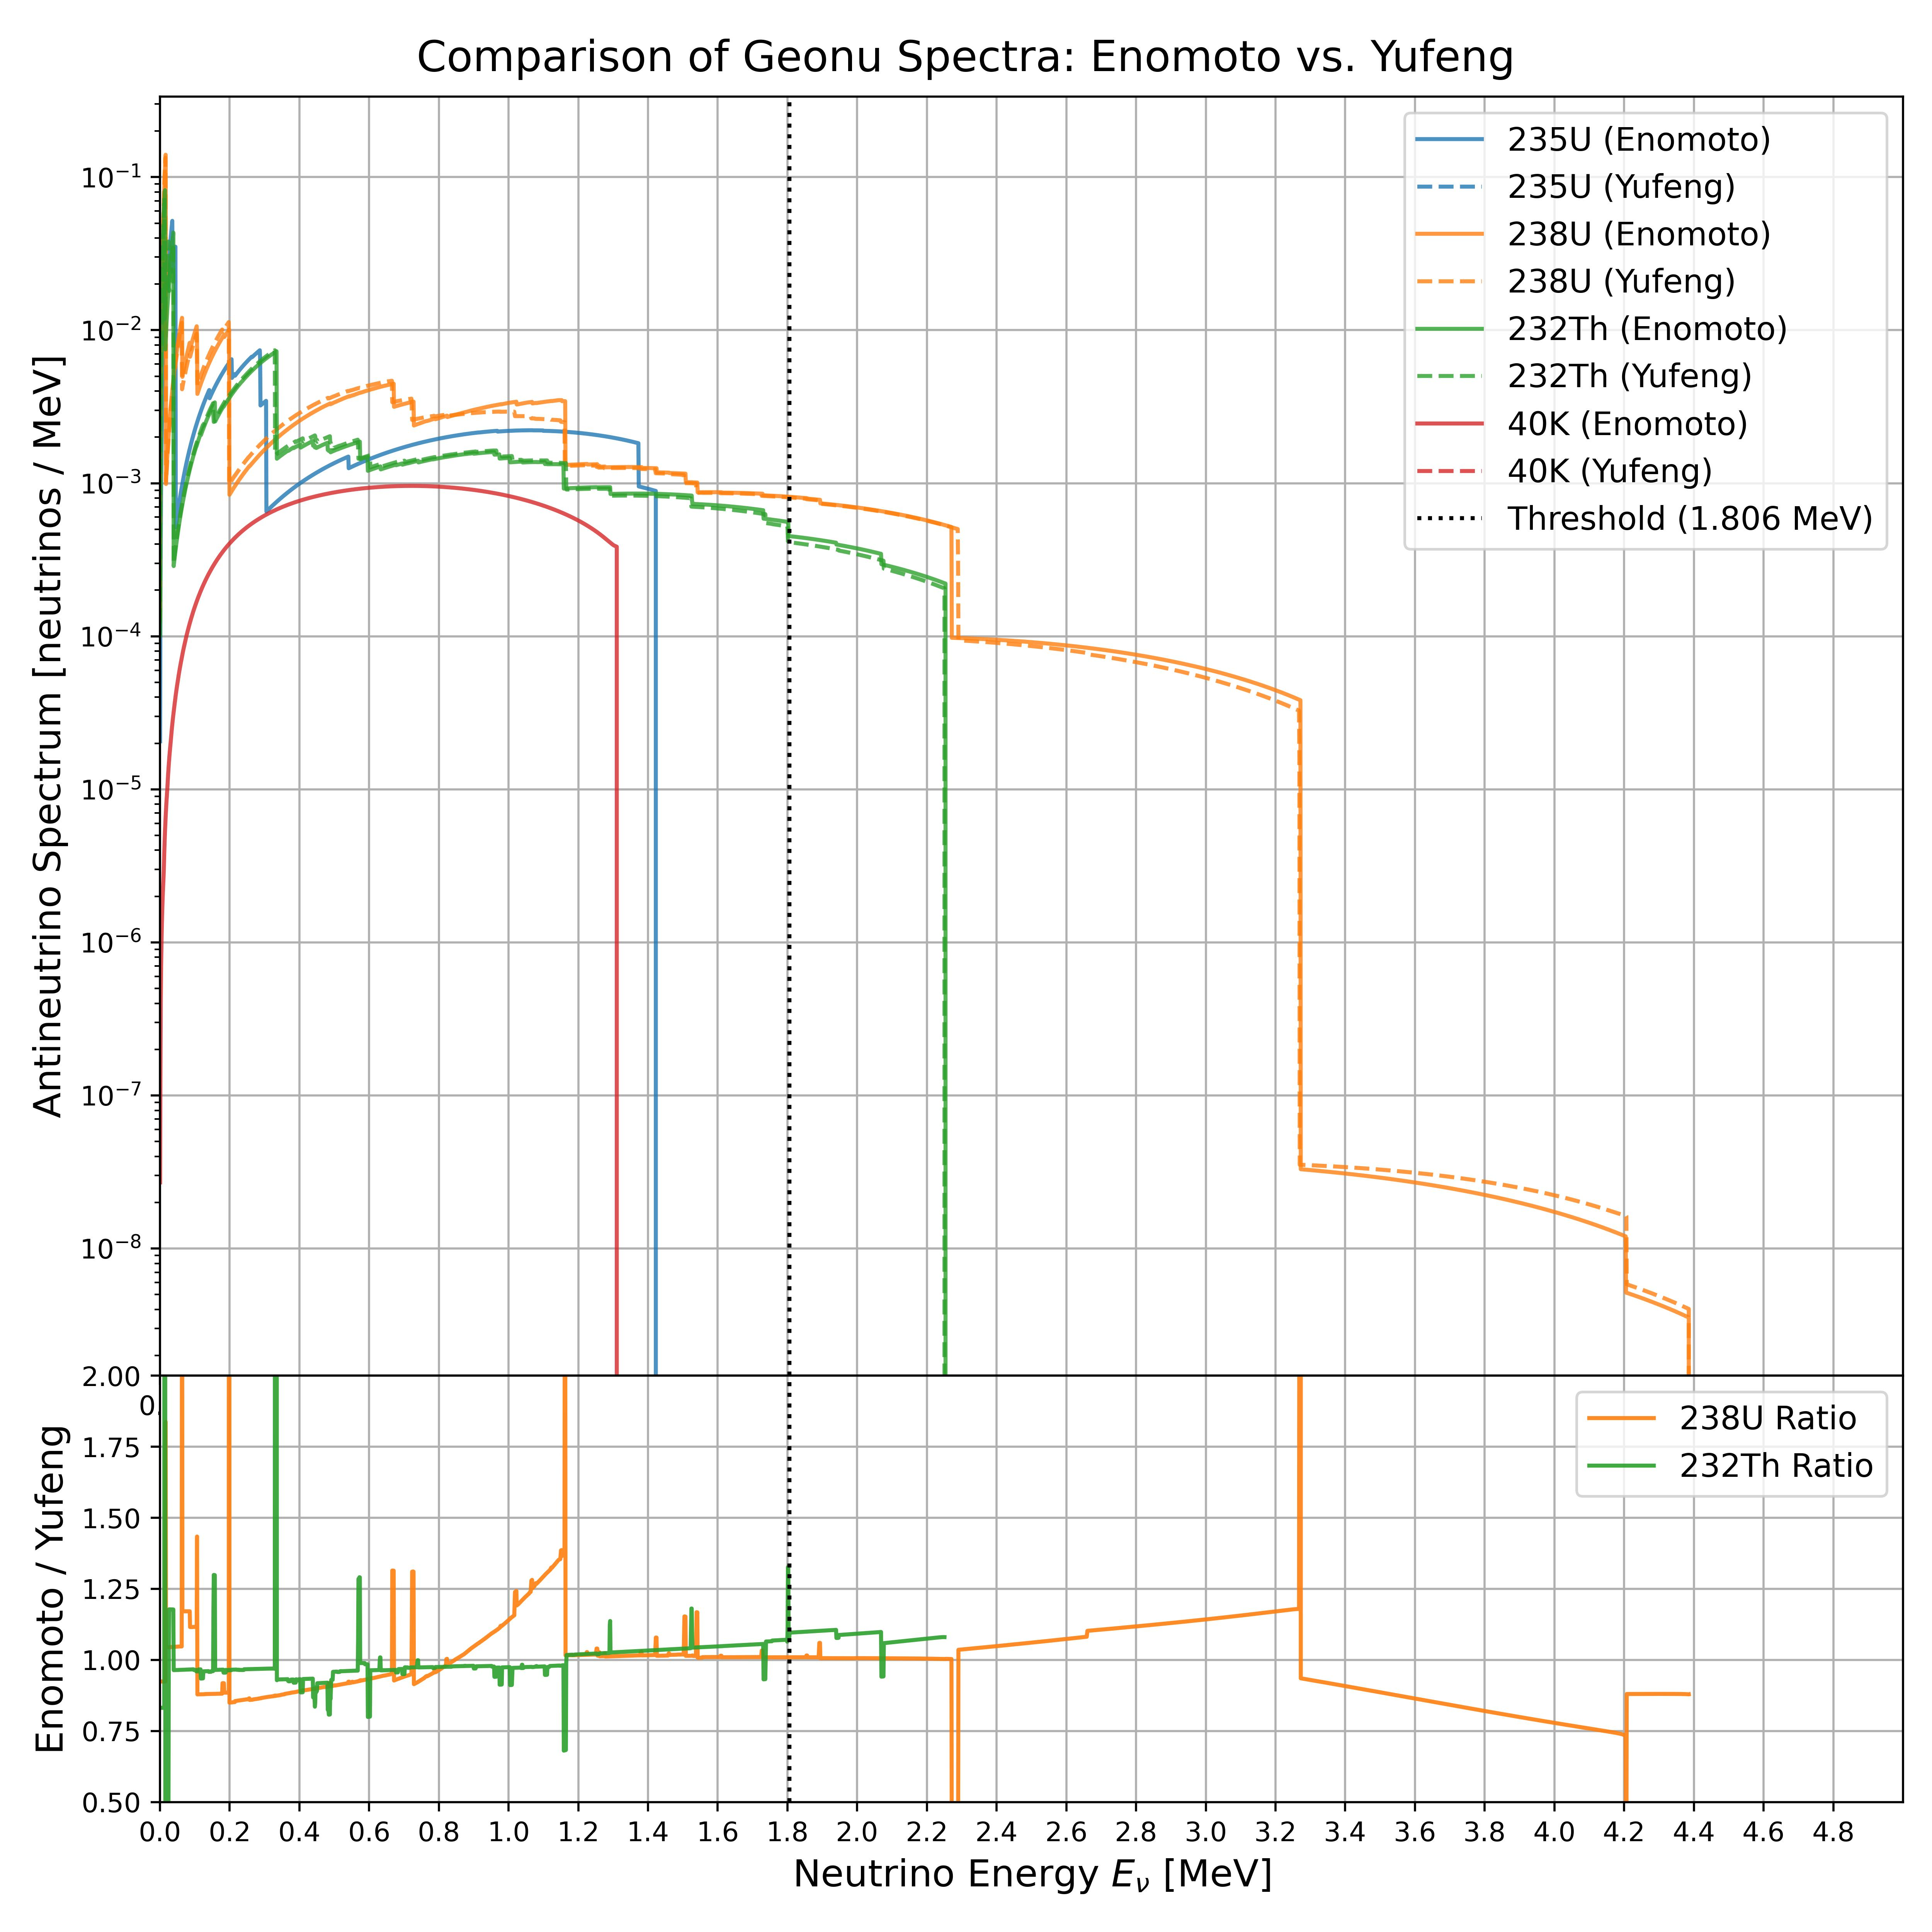
\includegraphics[scale = 0.3]{./Pics/Comparison_of_All_Geonu_Spectra.jpg}
					\caption{不同HPE元素衰变的地球中微子能谱\cite{Enomoto_Spectrum, GeonSpectra-2024}}
					\label{Fig:Geonu Decay}
				\end{figure}
		\section{GEONU软件}
			GEONU是一款开源的MATLAB代码,目前由Tytrice Faison和Laura Sammon负责维护\cite{Original_GEONU},这款软件对地球进行建模并且能够计算各个探测器的地球中微子信号,除此之外还有geonu flux、热功率等信息。我在此基础上对整套代码进行了改写,提高了可读性、可维护性,做到了模块化,以便于后续SNO+对地球中微子问题的研究。\par
			GEONU将地球划分成三大部分:Lithsophere、Mantle和Core;由于Core对地球中微子信号几乎没有贡献,所以着重计算了来自Lithosphre和Mantle的信号。Lithosphere被划分成了7层,分别是sediment(s1, s2, s3), Crust(UC, MC, LC)和LM,每一层按照经纬度划分成了$1^\circ \times 1^\circ$的格子,总共$64,800$个格子,如Fig. \ref{Fig:Earth Structure 1}。Mantle部分则是划分成了两层,分别是DM和EM,每一层同样是$64,800$个格子。整体结构看见Fig. \ref{Fig:Earth Structure 2}
				\begin{figure}[H]
					\centering
					\begin{minipage}{0.49\linewidth}
						\centering
						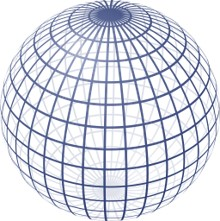
\includegraphics[width=0.6\linewidth]{./Pics/Earth_Structure_1.jpg}
						\caption{地层划分演示}
						\label{Fig:Earth Structure 1}
					\end{minipage}
					\begin{minipage}{0.49\linewidth}
						\center
						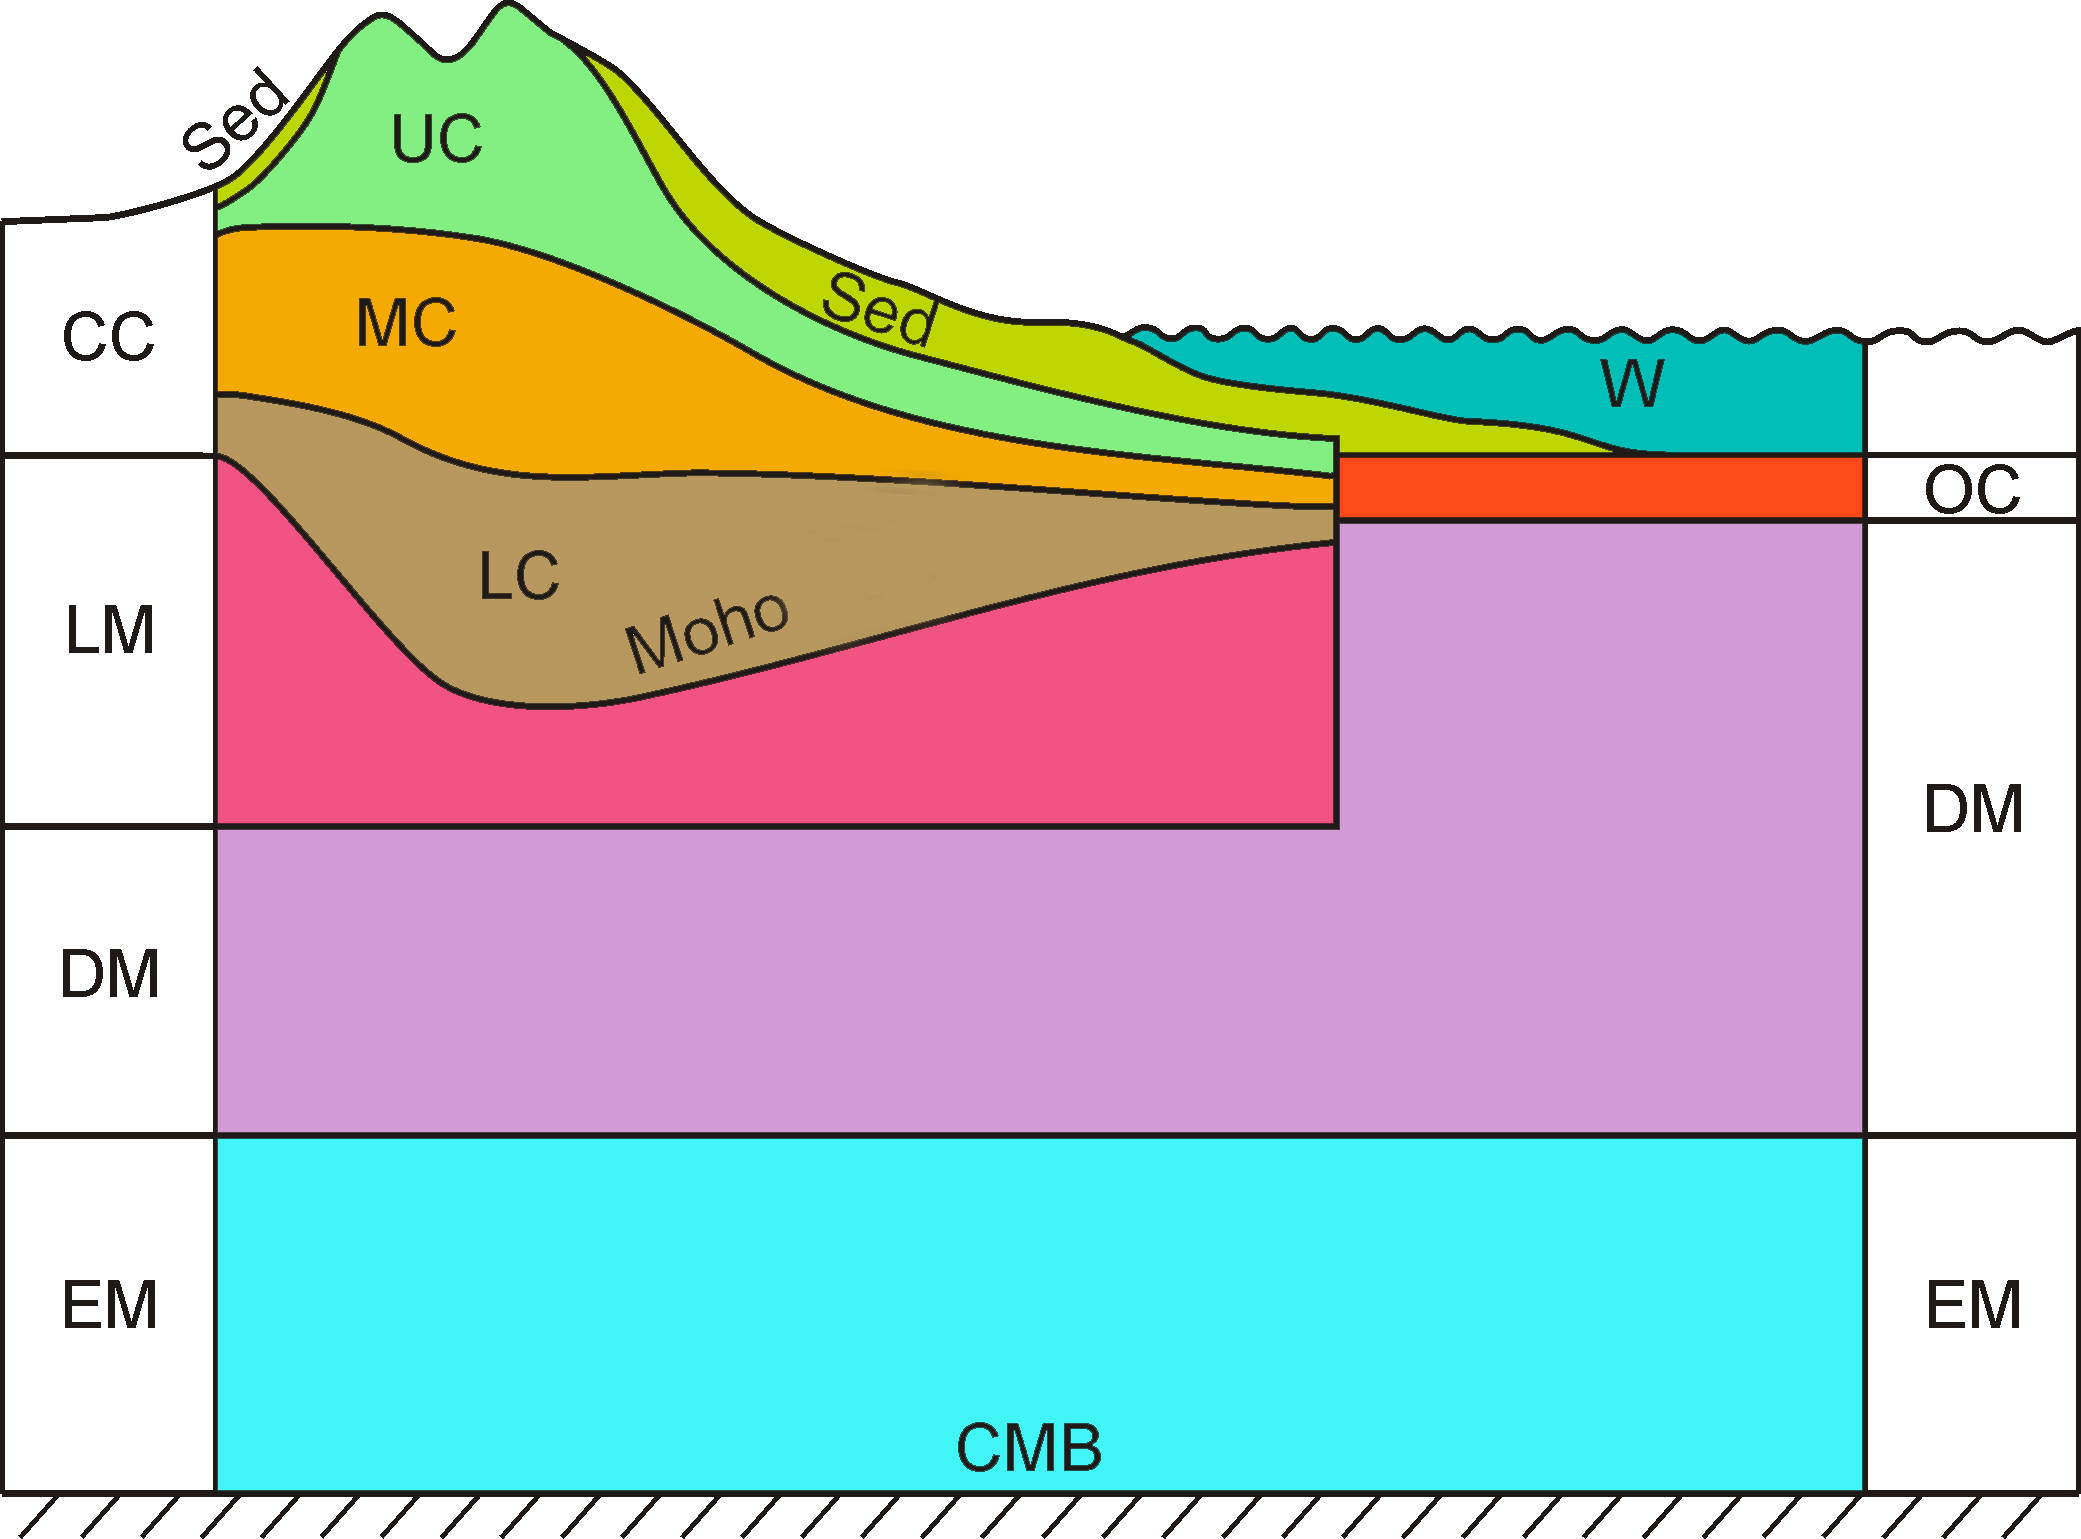
\includegraphics[width=0.8\linewidth]{./Pics/Earth_Structure_2.jpg}
						\caption{地球内部结构\cite{huang2013reference}}
						\label{Fig:Earth Structure 2}
					\end{minipage}
				\end{figure}
			除此之外,GEONU输入了不同的地质模型数据。Lithosphere可选择数据有Crust1.0, Crust2.0, Lith和ECM;Mantle导入的数据是PREM。目前,整个改写工作Lithosphere只支持Crust1.0模型。\par
			有了地球建模之后,接下来就是如何计算地球中微子信号。对于第$i$个HPE元素,其产生的信号为
				\begin{equation}
					S_i
					= \int_{\oplus} \rho A_i dV \times \frac{1}{a_i} \times \frac{\ln 2}{\tau_i}\times \int \frac{dn}{dE} \sigma_{IBD} dE \times \frac{P_{ee}}{4\pi L^2} \times 1 \text{yr} \times N_{proton} \times \varepsilon_{detector},
				\end{equation}
			其中$\rho$是岩石密度;$A_i, a_i, \tau_i$分别是第$i$个HPE元素的丰度、原子质量和半衰期;$P_{ee}$是存活概率;$L$是岩石到探测器的距离;$N_{proton}$是靶质子数;$\varepsilon_{detector}$是探测效率。通量的计算公式为
				\begin{equation}
					\Phi
					= \int_{\oplus} \rho A_i dV \times \frac{1}{a_i} \times \frac{\ln 2}{\tau_i}\times \int \frac{dn}{dE} dE \times \frac{P_{ee}}{4\pi L^2},
				\end{equation}
			其单位通常是cm$^{-2}$s$^{-1}$。热功率则是通过HPE元素质量直接计算。至此,整个GEONU计算框架到此结束,更加详细的细节和讨论将会放到后续章节当中。
		\section{如何使用GEONU?}
			如果你是第一次接触、使用GEONU软件的话,请首先安装MATLAB软件。安装完成之后,打开\textbf{main.mlx}文件,选择你关注的探测器,设置想要的迭代次数,然后点击程序运行。迭代次数和内存息息相关,请参考下列的推荐表格:
				\begin{table}[H]
					\centering
					\caption{不同迭代次数推荐内存及所需时间}
					\begin{tabular}{|c|c|c|}
						\hline
						迭代次数 & 推荐内存 & 所需时间\\
						\hline
						$1000$ & $32$ GB & $102$ s\\
						\hline
						$4000$ & $64$ GB & $280$ s\\
						\hline
					\end{tabular}
				\end{table}
			程序结束之后,结果会保存在\textbf{Output}文件夹。计算结果保存了三个structure:Physics、Geology和Output。前两个记录物理和地质输入,以便于后续检查和复现;Output记录计算结果。\textbf{Plot.m}文件展示了如何读取、展示计算结果,所有输出图片都会保存在\textbf{Pics}文件夹当中。\par
			\texttt{LITE}版本展示了计算的基本框架,后续的\texttt{ADVANCE}和\texttt{SPECTRUM}都是基于此发展而来,只不过是为了控制内存消耗而做了对应的特异化处理。如果你想要对此进行改进或者拓展的话,\texttt{LITE}由于高度模块化、数据结构清晰所以将会是一个非常好的参考例子。针对内存消耗,目前针对不同的功能开发了不同的版本:
				\begin{itemize}
					\item \textbf{LITE:}只关注与事例率的计算。
					\item \textbf{ADVANCE:}同时计算事例率、signal flux和热功率。
					\item \textbf{SPECTRUM:}计算事例率与测量能谱。
					\item \textbf{APPLICATION:}自定义开发与应用。
				\end{itemize}
			{\color{red} 注:如果您的文章中有任何基于新版或者旧版GEONU的结论或者论点的话,请引用这篇文献\cite{wipperfurth2020reference},它是第一个提供此代码的论文。}
	\chapter{地质相关信息(TBA)}
		\section{Huang方法}
		\label{Geology: Huang Method}
			Huang方法基于~\cite{Huang2013}。这个方法基于以下地质学证据:1)地质学观察到了地震波速$V_p$和$V_s$和岩石中SiO$_2$的含量成反比;2)由于MC和LC的温度和压强的关系,这两个岩层的主要成分分别是amphibolite和granulite。同时,每一类岩石都可以根据SiO$_2$的含量分成felsic,intermediate和mafic三类。Huang等人就假设amphibolite和granulite由felsic和mafic两类构成,比例分别是$f,m$,然后测量了这两类岩石的$V_p$,最后通过线性组合去匹配真实测量结果$V_\mathrm{crust}$。也就是求解如下方程组:
				\begin{equation}
					f + m = 1,
					\quad
					fV_{f, p} + mV_{m, p}
					= V_\mathrm{crust}.
				\end{equation}
			最后利用felsic和mafic两类演示的丰度,通过线性组合
				\begin{equation}
					a = fa_f + ma_m
				\end{equation}
			给出MC和LC岩层的丰度。元素的丰度服从Log-Gaussian分布,而不是高斯分布。GEONU中会利用以下数据
				\begin{table}[H]
					\centering
					\caption{Huang方法中丰度输入}
					\begin{tabular}{c|c|c|c|c|c|c|c|c|c}
						\hline
						\hline
						Rock & $\mu_\mathrm{U}$(ppm) & $+\Delta_\mathrm{U}$ & $-\Delta_\mathrm{U}$ & $\mu_\mathrm{Th}$(ppm) & $+\Delta_\mathrm{Th}$ & $-\Delta_\mathrm{Th}$ & $\mu_\mathrm{K_2O}$ (wt\%)& $+\Delta_\mathrm{K_2O}$ & $-\Delta_\mathrm{K_2O}$\\
						\hline
						Amphibolite: Felsic & $1.37$ & $1.03$ & $0.59$ & $8.27$ & $8.12$ & $4.10$ & $2.89$ & $1.81$ & $1.11$\\
						\hline
						Amphibolite: Mafic & $0.37$ & $0.39$ & $0.19$ & $0.58$ & $0.57$ & $0.29$ & $0.50$ & $0.41$ & $0.23$\\
						\hline
						Granulite: Felsic & $0.42$ & $0.41$ & $0.21$ & $0.387$ & $7.35$ & $2.54$ & $2.71$ & $2.05$ & $1.17$\\
						\hline
						Granulite: Mafic & $0.10$ & $0.14$ & $0.06$ & $0.30$ & $0.46$ & $0.18$ & $0.39$ & $0.31$ & $0.17$\\
						\hline
						\hline
					\end{tabular}
				\end{table}
				\begin{figure}[H]
					\centering
					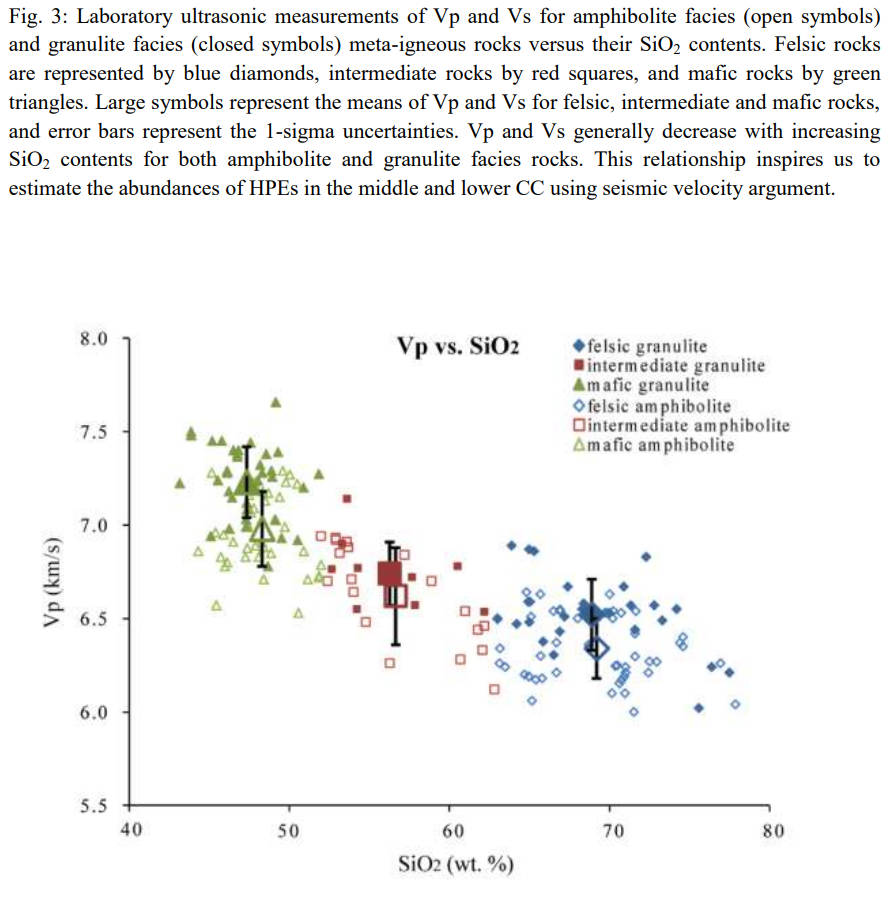
\includegraphics[scale = 0.27]{./Pics/Pic-Vp_SiO2.jpg}
					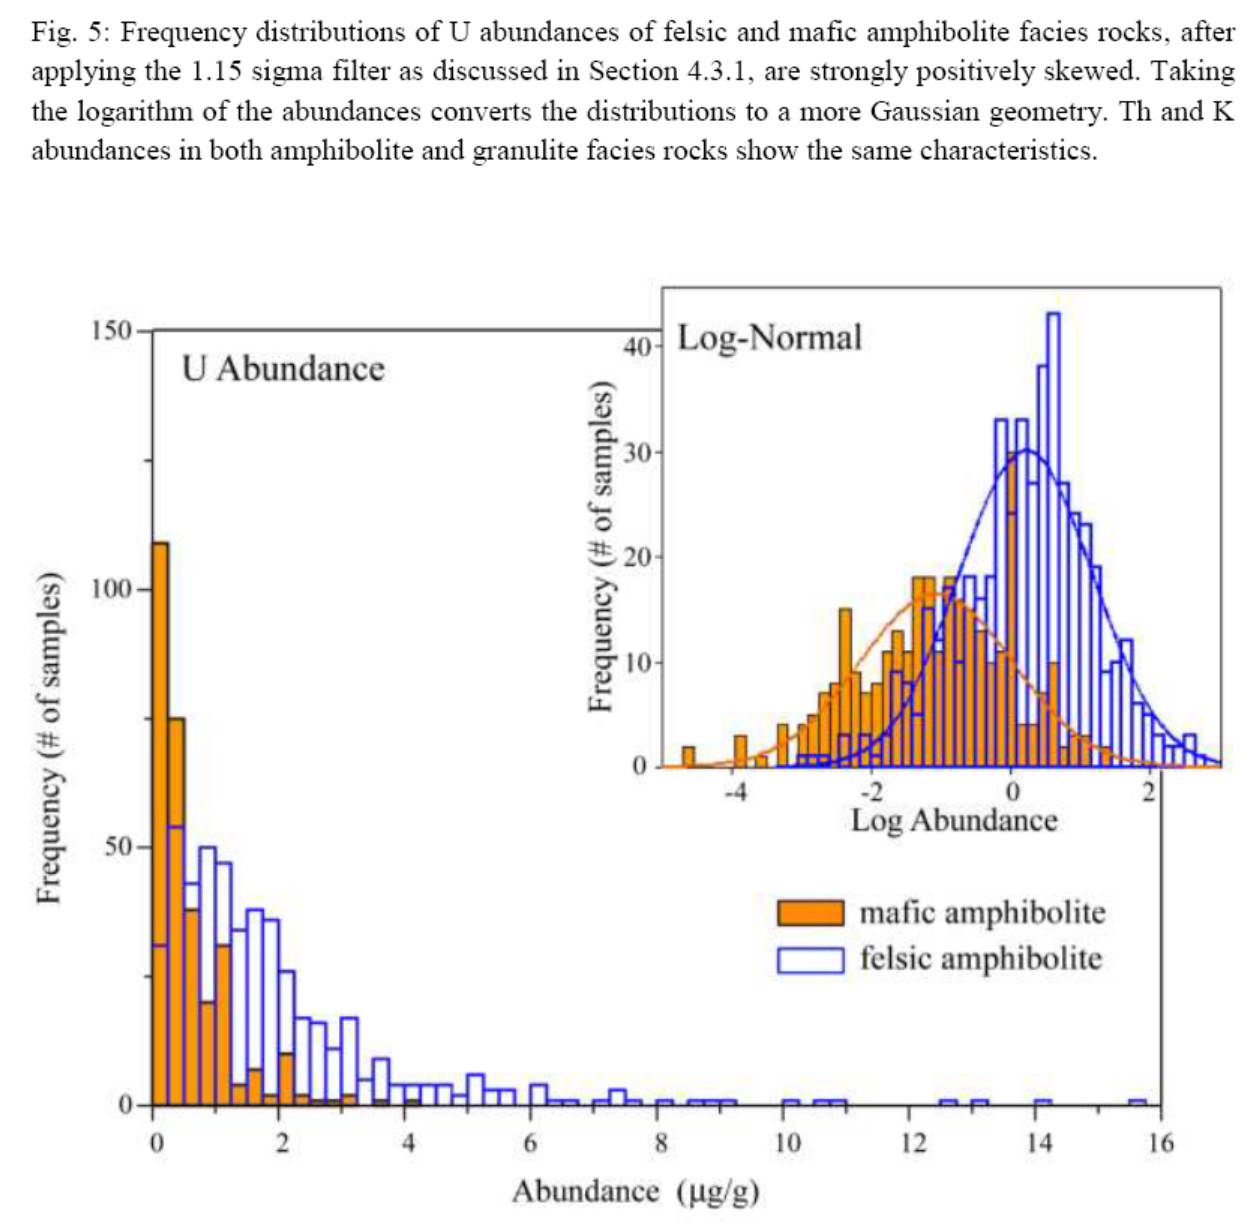
\includegraphics[scale = 0.2]{./Pics/Pic-Abundance_Distribution.jpg}
				\end{figure}
		\section{Bivart方法}
		\label{Geology: Bivart Method}
		\section{Crust 1.0}
		\section{Crust 2.0}
		\section{Litho 1}
		\section{ECM}
		
	\chapter{输入参数}
		\section{物理输入}
			物理输入主要有:
				\begin{enumerate}
					\item \textbf{元素性质:}详见表格\ref{Table: Element Properties}
					\item \textbf{中微子振荡:}振荡参数详见表格\ref{Table: Oscillation Parameters};振荡公式为
						\begin{equation}
							\begin{aligned}
								P_{ee}(E, L)
								= 1  
								&- \sin^2 2\theta_{12}\cos^4 \theta_{13} \sin^2\left(\frac{1.27 \Delta m_{21}^2 L}{E}\right) \\
								&- \sin^2 2\theta_{13}\cos^2 \theta_{12} \sin^2\left(\frac{1.27 \Delta m_{31}^2 L}{E}\right) \\
								&- \sin^2 2\theta_{13}\sin^2 \theta_{12} \sin^2\left(\frac{1.27 \Delta m_{32}^2 L}{E}\right),
							\end{aligned}
						\end{equation}
					其中$E, L$的单位分别为MeV和km。
					\item \textbf{HPE元素衰变的中微子能谱:}目前Geonu领域的研究普遍采用的能谱是Enomoto计算提供的\cite{Enomoto_Spectrum}。李玉峰考虑了紧闭跃迁以及高阶修正,给出了更加精细的能谱~~\cite{GeonSpectra-2024}。两个能谱可见图\ref{Fig:Geonu Decay}。新的能谱会导致到更少的地球中微子信号,U会减少$3.47\%$,Th会减少$9.00\%$。
						\begin{figure}[H]
							\centering
							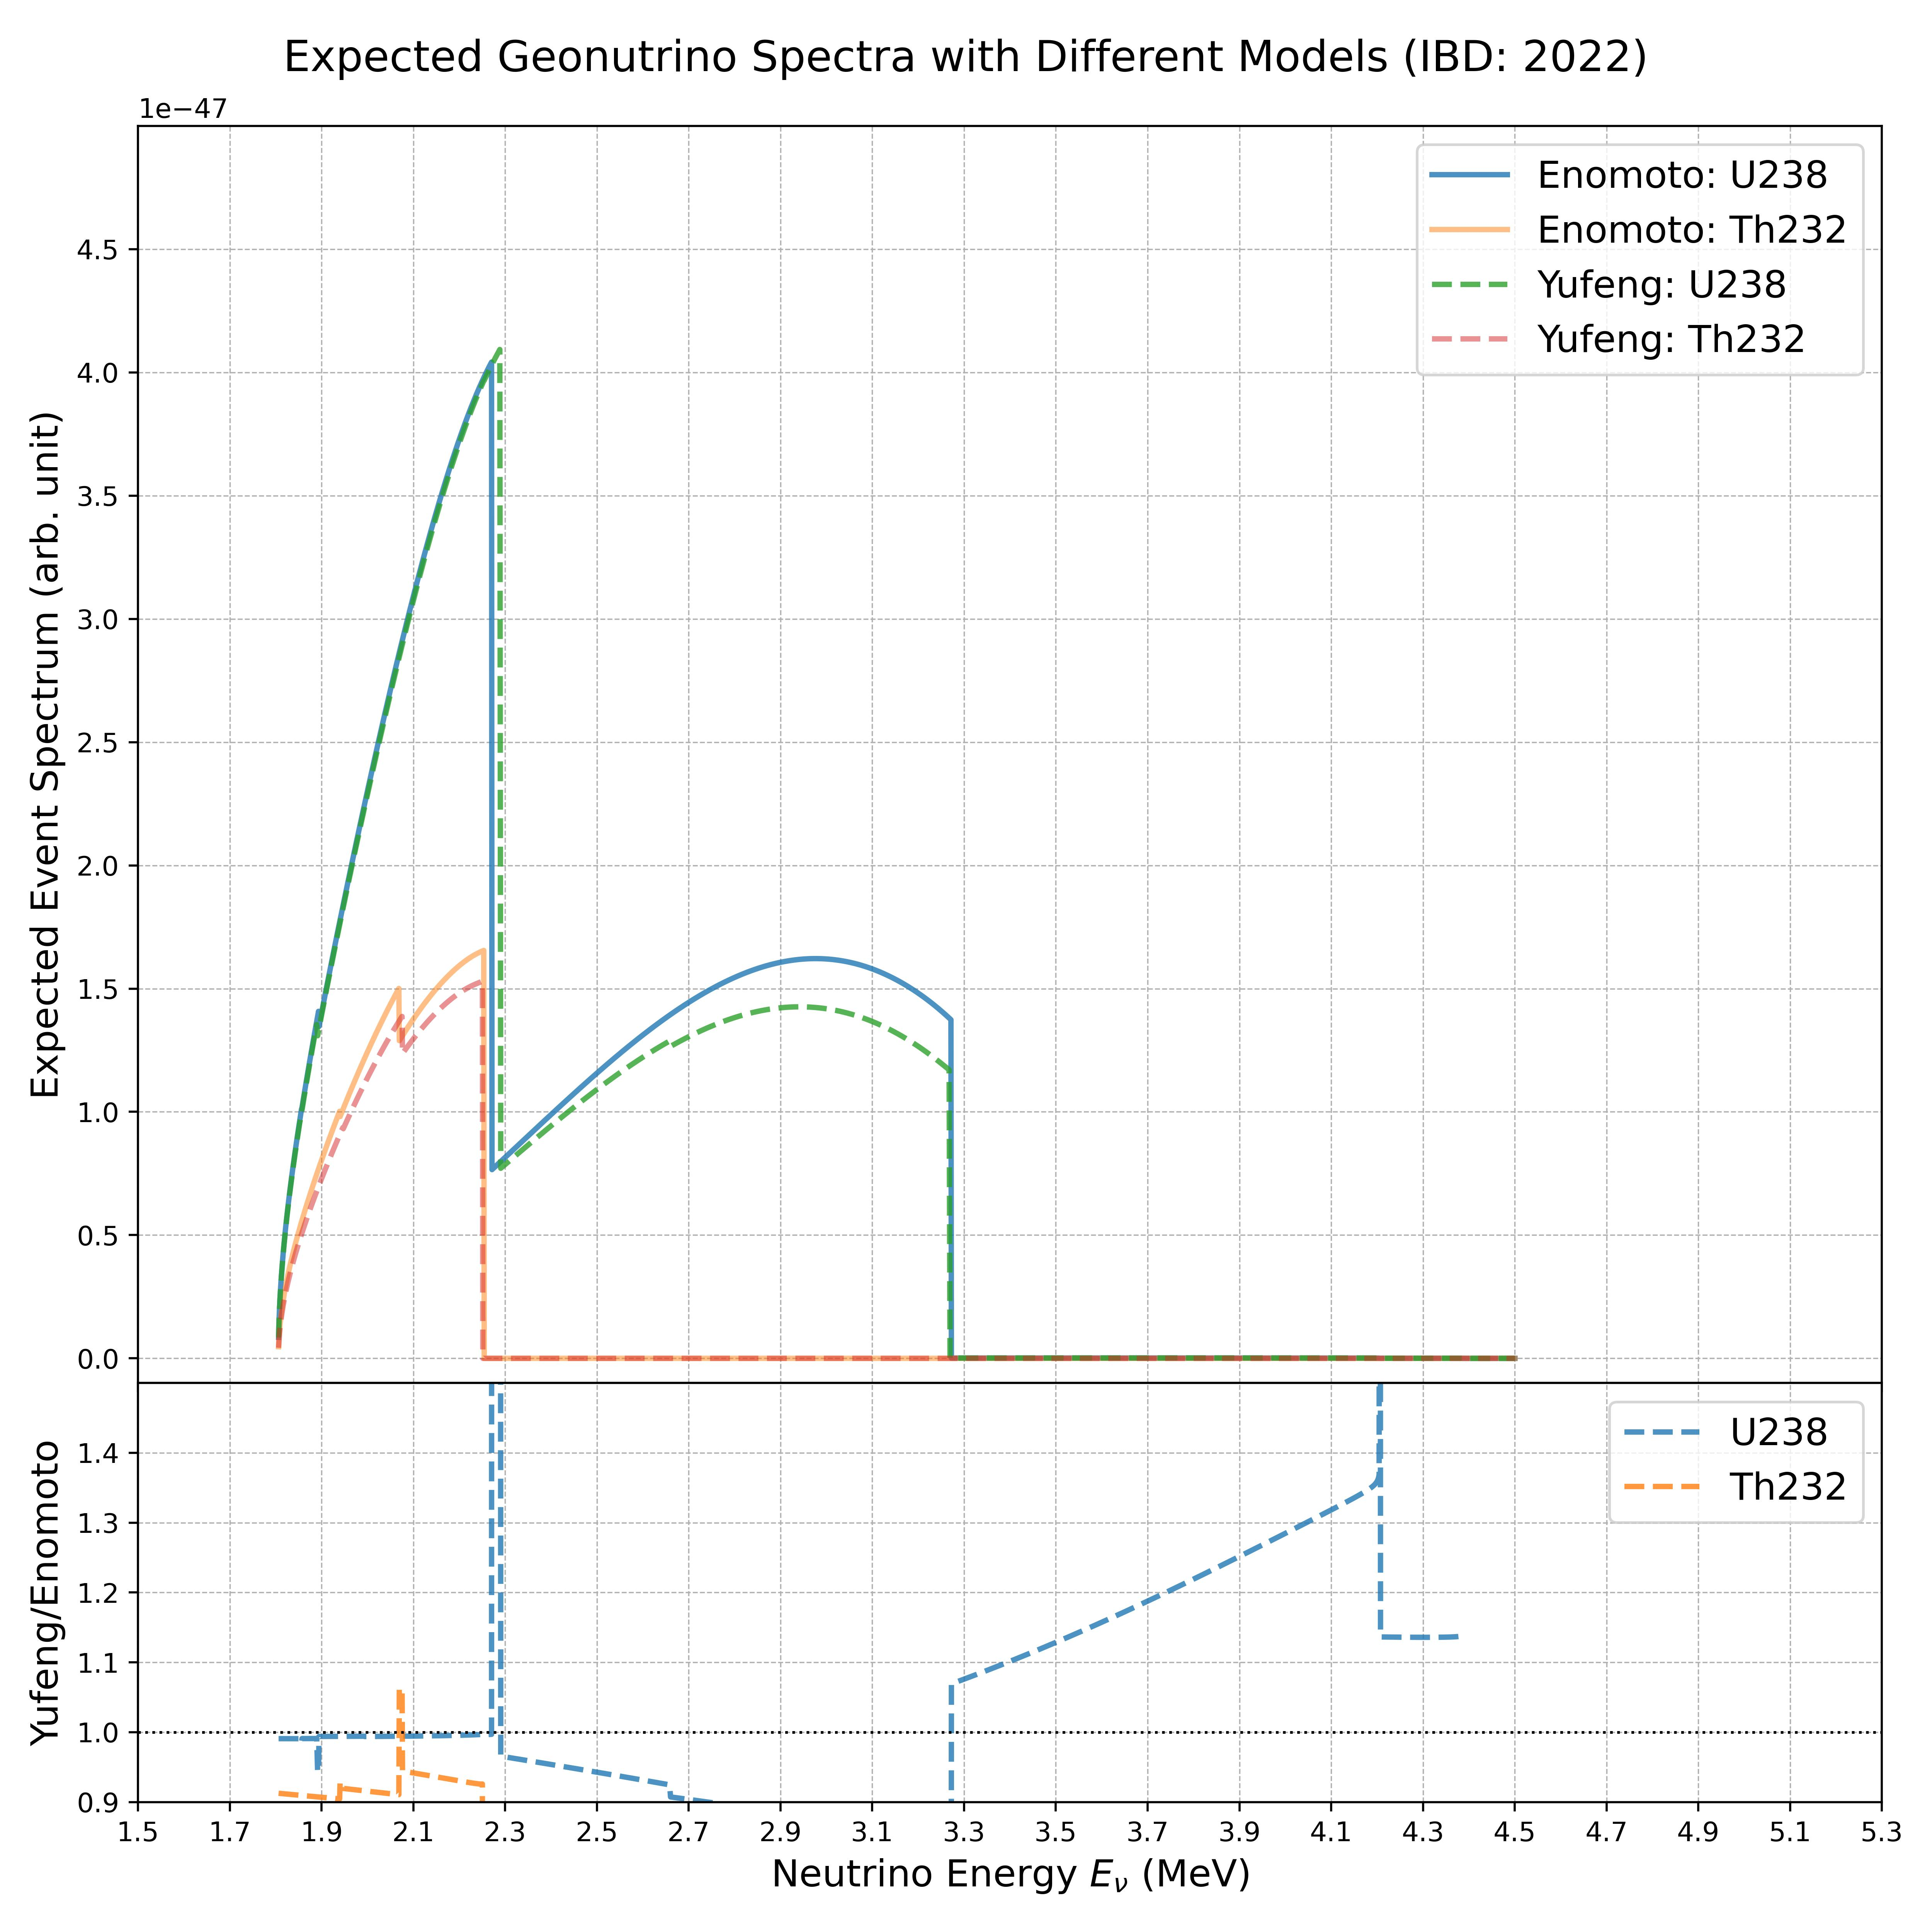
\includegraphics[scale = 0.5]{./Pics/Comparison_All_Expected_Geonu_Spectra_IBD_2022.jpg}
						\end{figure}
					\item \textbf{IBD散射截面:}GEONU支持四种IBD散射截面,所有截面都存储到了\texttt{./Input\_Files/IBD\_Cross\_Section.mat}中,分别是:\par
					1)\texttt{Approximation}:这是geonu建模研究中最常用的公式,具体为:
						\begin{equation}
							\sigma_{IBD}(E)
							= 9.52 \times (E - \Delta)^2 \sqrt{1 - \frac{m_e^2}{(E - \Delta)^2}} \times 10^{-44} \text{cm}^2,
						\end{equation}
					其中$\Delta \equiv m_n - m_p \approx 1.2933$ MeV。\par
					2) \texttt{Vogel \& Beacom (1999)}: 这个计算基于~\cite{IBD-1999}。这篇文章考虑了nucleon recoil和weak magnetism,并且用$M\rightarrow\infty$进行泰勒展开给出了保留到一阶的渐近公式。\par
					3) \texttt{Strumia \& Vissani (2003)}:这个计算基于~\cite{IBD-2003}。这篇文章考虑了$f_1, f_2, g_1, g_2$四种形状因子进行了完整的相对论计算,并且估计了低能区的散射截面误差大概为$0.4\%$。\par 
					4) \texttt{Vissani et al. (2022)}:这个计算基于~\cite{IBD-2022}。这篇文章考虑了$f_3, g_3$形状因子产生的Second-class current,并且估计了低能区的散射截面误差大概为$0.094\%$。
						\begin{figure}[H]
							\centering
							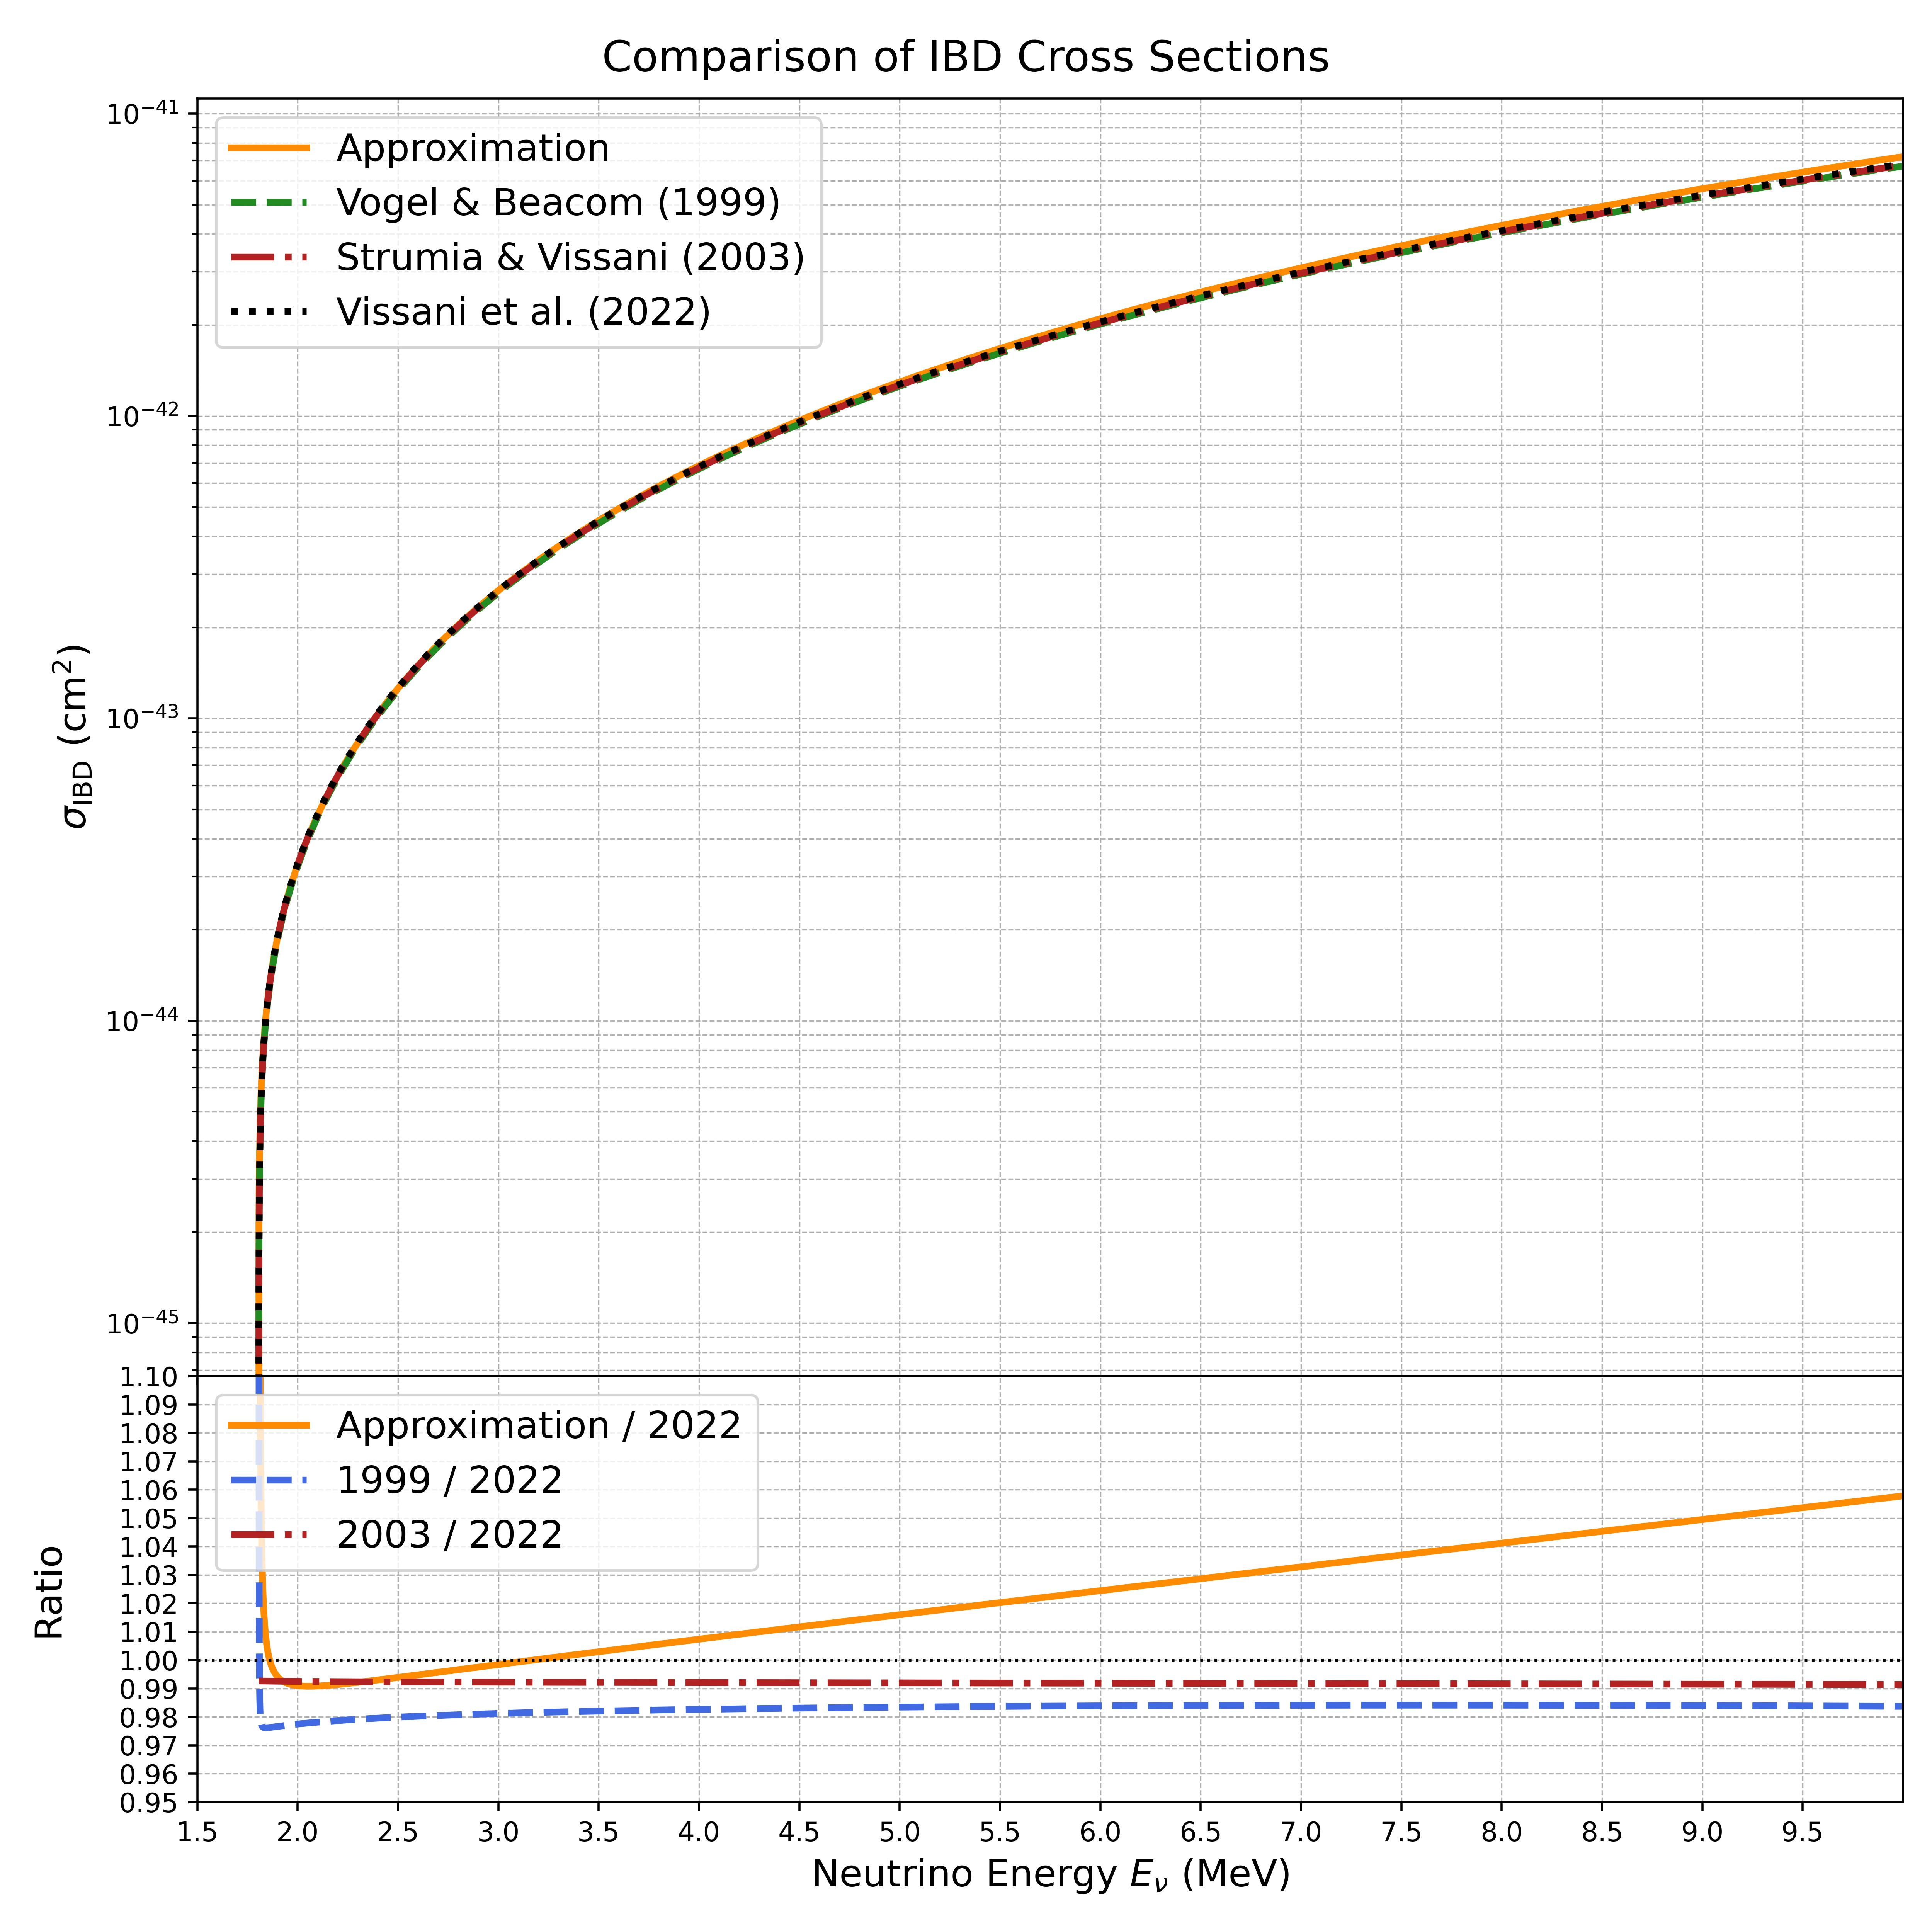
\includegraphics[scale = 0.5]{./Pics/Comparison_of_All_Computed_IBD_Cross_Section.jpg}
						\end{figure}
				\end{enumerate}
				\begin{table}[H]
					\centering
					\caption{元素性质}
					\begin{tabular}{p{3.5cm}|p{2cm}p{2cm}p{2cm}p{3cm}|p{2cm}}
						\hline
						\hline
						性质 & ${}^{235}U$ & ${}^{238}U$ & ${}^{232}Th$ & ${}^{40}K$ & 来源\\
						\hline
						自然丰度 & $0.7\%$ & $99.3\%$ & $100\%$ & $0.0117\%$ & Wiki\\
						\hline
						原子质量(amu) & $235.0439299$& $238.05078826$ & $232.0380536$ & $39.96399848165$ & Wiki \\
						\hline
						半衰期(s)/$3.1536$e$7$ & $4.468$e$9$ & $0.704$e$9$ & $14.05$e$9$ & $1.248$e$9$ & Wiki \\
						\hline
						反射热$\mu$W/kg & $568.48$ & $95.13$ & $26.28$ & $24.47$ & Ref \cite{dye2012geoneutrinos}\\
						\hline
						\hline
					\end{tabular}
					\label{Table: Element Properties}
				\end{table}
				\begin{table}[H]
					\centering
					\caption{中微子振荡 (PDG 2024)}
					\begin{tabular}{p{2cm}|p{3cm}|p{3cm}|p{3cm}}
						\hline
						\hline
						混合角 & 数值 & 质量差($\text{eV}^2$) & 数值\\
						\hline
						$\sin^2 \theta_{13}/10^{-2}$ & $2.203\pm 0.059$ & $\Delta m_{21}^2/10^{-5}$ & $7.41\pm 0.21$\\
						\hline
						$\sin^2 \theta_{12}/10^{-1}$ & $3.03\pm 0.12$ & $\Delta m_{31}^2/10^{-3}$ & $2.437\pm 0.028$\\
						\hline
						$\sin^2 \theta_{23}/10^{-1}$ & $5.72\pm 0.23$ & $\Delta m_{32}^2/10^{-3}$ & $2.437\pm 0.028$\\
						\hline
						\hline
					\end{tabular}
					\label{Table: Oscillation Parameters}
				\end{table}
				\begin{table}[H]
					\centering
					\caption{电子与核子质量}
					\begin{tabular}{p{3cm}p{3cm}p{3cm}|p{3cm}}
						\hline
						\hline
						$m_e$(MeV) & $m_p$(MeV) & $m_n$(MewV) & 来源\\
						\hline
						$0.51099895069$ & $938.27208943$ & $939.56542052$ & Wiki\\
						\hline
						\hline
					\end{tabular}
					\label{Table: Electron and Nucleon Mass}
				\end{table}
		\section{地质输入}
			地质学方面的输入包括以下几部分
				\begin{enumerate}
					\item \textbf{Lithosphere的地质数据:}目前仅支持Crust 1.0;未来会逐渐支持Crust 2.0, Litho 1.0和ECM1模型。这些模型会提供岩石密度、深度、厚度等信息。
					\item \textbf{Lithosphere的HPE元素丰度:}需要输入U、Th和K元素丰度的平均值和对应误差,软件会自动根据平均值和误差随机抽样出每个格子的元素丰度;其中MC和LC的CC部分则是采用Huang或者Bivart的方法自动计算丰度。
					\item \textbf{Mantle的地质数据:}PREM模型,可以提供不同深度地层的密度信息。
					\item \textbf{Mantle的丰度信息:}DM地层U的丰度、Th/U和K/Th丰度比值;以及BSE模型的U丰度和Th/U和K/Th丰度比值。
					\item \textbf{其他参数:}计算过程中用到的其他参数。
				\end{enumerate}
				\begin{table}[H]
					\centering
					\caption{Lithosphere中各地层的默认丰度}
					\renewcommand{\arraystretch}{1.2} % 增加表格行距
					\begin{tabular}{p{1.5cm}|p{2cm}p{2cm}p{3cm}|p{2cm}p{2cm}p{3cm}}
						\hline
						\hline
						\multirow{2}{*}{地层} & \multicolumn{3}{c|}{CC} & \multicolumn{3}{c}{OC} \\  
						\cline{2-7}
						& U/$10^{-6}$ & Th/$10^{-6}$ & K/$10^{-2}$ & U/$10^{-6}$ & Th/$10^{-6}$ & K/$10^{-2}$\\
						\hline
						Sediment & $1.73\pm 0.09$ & $8.10\pm 0.59$ & $(2.21 \pm 0.14)* 0.83$ & $1.73 \pm 0.09$ & $8.10 \pm 0.59$ & $(2.21 \pm 0.14) * 0.83$\\
						\hline
						UC & $2.7 \pm 0.6$ & $10.5 \pm 1.0$ & $2.32 \pm 0.19$ & $0.07\pm 0.021$ & $0.21 \pm 0.063$ & $0.0716 \pm 0.0215$\\
						\hline
						MC/LC & \multicolumn{3}{c|}{Huang/Bivart} & $0.07 \pm 0.021$ & $0.21 \pm 0.063$ & $0.0716 \pm 0.0215$ \\
						\hline
						LM & $0.033^{+0.049}_{-0.020}$ & $0.15^{+0.277}_{-0.097}$ & $0.0315^{+0.04316}_{-0.01826}$ & \multicolumn{3}{c}{$0$} \\
						\hline
						\hline
					\end{tabular}
					\label{Table: Lithosphere Default Abundance Input}
				\end{table}
				\begin{table}[H]
					\centering
					\caption{BSE默认丰度}
					\begin{tabular}{p{3cm}p{3cm}p{3cm}}
						\hline
						\hline
						U/$10^{-9}$ & Th/U & K/U\\
						\hline
						$19 \pm 3.8$ & $3.776^{+0.122}_{-0.075}$ & $13800 \pm 1300$\\
						\hline
						\hline
					\end{tabular}
					\label{Table: BSE Default Abundance Input}
				\end{table}
				\begin{table}[H]
					\centering
					\caption{地幔默认输入}
					\begin{tabular}{p{3cm}p{3cm}p{3cm}}
						\hline
						\hline
						EM(质量)占比 & Th/U & K/U \\
						\hline
						$19\%$ & $3.45^{+1.66}_{-1.18}$ & $19000 \pm 1300$\\
						\hline
						\hline
					\end{tabular}
				\end{table}
				\begin{table}[H]
					\centering
					\caption{其他默认输入}
					\begin{tabular}{p{4cm}|p{4cm}}
						\hline
						\hline
						地球质量(kg)/$10^{24}$ & 地核质量(kg)/$10^{24}$\\
						\hline
						$5.97218 \pm 0.00006 $ & $ 1.93265 \pm 0.0579795$\\
						\hline
						\hline
					\end{tabular}
					\label{Table: Other Default Geology Input}
				\end{table}
		\section{三种BSE模型的地质参数输入(TBA)}
	\chapter{软件设计}
		\section{软件设计思想}
			\subsection{抽样}
				GEONU的程序设置当中有一个重要的概念就是通过随机抽样引入不确定性,具体通过以下两个函数实现:
					\begin{enumerate}
						\item \texttt{Generate\_Random\_Normal():}高斯抽样
						\item \texttt{Generate\_Random\_Log\_Normal():}Log高斯抽样
					\end{enumerate}
				这些抽样方式使得GEONU能在计算过程充分考虑不确定性,并将其最终传播到最终结果当中。同时,GEONU通过关联系数的方式来建立不同输入变量的相关性,从而实现了更真实、物理的模拟。
			\subsection{统计与误差}
				在原有GEONU程序的\texttt{Abund\_And\_Flux()}当中,计算完成之后会调用\texttt{stat()}等函数给出统计相关的结果,但这种方法即会严重拖慢程序的运行还破坏了整体结果的随机性。基于此,新版GEONU彻底删除了计算过程中所有的统计的内容,在后续分析中只对最后的整体运算结果采用统计学处理。具体应用可以查看\texttt{./Plot.m}。
		\section{物理}
			所有和物理相关的函数都放到了\texttt{./Functions/Physics}当中。它们的名字和功能分别是:
				\begin{enumerate}
					\item \texttt{Compute\_Relative\_Abundance\_Mass():}此函数利用元素的自然丰度计算了质量丰度。以U元素为例,GEONU软件输入和计算的丰度都是U这个元素的总丰度,而U却包含${}^{238}$U,${}^{235}$U和${}^{234}$U;利用此丰度就可以从总丰度中计算出${}^{238}$U的贡献。
					\item \texttt{Load\_Oscillation\_Parameters():}默认振荡参数会存储在这里,并且可以通过\texttt{Physics.Oscillation.Constant}来判断是否对振荡参数进行随机抽样,不过目前这个功能不打算启用。程序的最后还计算了\texttt{p1, p2, p3}三个变量,它们分别是
						\begin{align}
							 p1 = -\sin^2 2\theta_{12} \cos^4 \theta_{13},
							 \quad
							 p2 = -\sin^2 2\theta_{13} \cos^2 \theta_{12},
							 \quad
							 p3 = - \sin^2 2\theta_{13} \sin^2 \theta_{12},
						\end{align}
					这三个变量会简化中微子振荡的代码,便于维护和理解。
					\item \texttt{Load\_Geonu\_Spectrum():}此函数用来加载HPE元素衰变的中微子能谱。原能谱的单位分别是keV和1/keV,为了加速计算同时考虑到能量分辨率,将原能谱进行了整合,目前只考虑$0-3.5$MeV范围的能谱,bin宽$0.1$MeV。
					\item \texttt{Compute\_Cross\_Section():}此函数用来导入IBD散射截面。
					\item \texttt{Compute\_Signal\_Response():}此函数计算了${}^{238}$U和${}^{232}$Th的signal rate response, $g_i$,其定义为:
						\begin{equation}
							G_i
							\equiv \frac{1}{4\pi}\frac{1}{a_i} \frac{\ln(2)}{\tau_i} \left(\frac{dn}{dE}\right) \sigma_{IBD} \times 1 \textbf{yr} \times 10^{32} \times \frac{1}{10^4},
						\end{equation}
					其中$10^{-4}$来自于$cm^2\rightarrow m^2$的单位换算。于是Geonu signal的计算公式简化为
						\begin{equation}
							S
							= \int_{\oplus} \rho A_i dV \times g_i \times \frac{P_{ee}}{L^2}.
						\end{equation}
					\item \texttt{Load\_Detector():}加载对应探测器的信息。每一条探测器的数据格式为:1) 经度;2) 纬度;3) 深度(m);4) 探测效率;5) 质子数;6) 距离探测器最近的格子的经纬度;7) 名称。
				\end{enumerate}
		\section{Lithosphere}
			所有与Lithosphere相关的脚本和函数放到了\texttt{./Functions/Geology},\texttt{./Functions/Computation/Lithosphere}和\texttt{./Functions/Computation/DeepCrust}。前者涉及到计算前的地质输入,后两者涉及到具体计算细节。\par
			\texttt{./Functions/Geology/Setting\_Asign.m}脚本记录了Lithosphere各个地层丰度的输入,几乎调用了\\
			\texttt{./Functions/Geology}下的所有函数,它们的名字及其作用为:
				\begin{enumerate}
					\item \texttt{Load\_Lithosphere\_Data():}这个函数首先会导入指定的地质模型;然后调用\texttt{Assign\_OC\_CC()},根据不同的模型首先对格子进行分类,指定哪些格子是CC部分哪些是OC部分。CC和OC的划分关系着后续元素丰度的指定和信号的计算方法;最后调用\texttt{Preallocate\_Variables\_Lithosphere()},规定每一层HPE元素的数据格式:每一行代表一个格子,总共有三列。它们分别代表着1)平均值;2)正误差;3)负误差。
					\item \texttt{Generate\_Correlations():}这个函数会产生所有抽样所需要的关联系数。其中所有地层的厚度的关联系数是一样的。Bivart方法中关于SiO${}_2$的关联系数集中到了\texttt{Generate\_Correlations\_DeepCrust()}中。
					\item \texttt{Compute\_Abundance\_DeepCrust():}这个函数会产生Huang方法所用数据,以及导入Bivart方法需要的数据。需要注意的是Huang方法K元素丰度采用的是K${}_2$O的重量百分比(wt\%),需要通过\texttt{wt}和\texttt{K2O}将最后计算结果转换成K元素丰度。
					\item \texttt{Assign\_Abundance\_Layer():}这个函数会指定所有格子的HPE丰度。
					\item \texttt{Compute\_Abundance\_BSE():}这个函数计算了BSE模型的HPE元素丰度。
					\item \texttt{Find\_Near\_Cells():}这个函数用来寻找探测器附近的格子,但未来不考虑采用这个函数。
				\end{enumerate}
			\par
			\texttt{./Functions/Computation/Lithosphere/Generate\_Temp\_Variables\_For\_Parallel.m}这个脚本定义计算过程中需要的变量,其中定义了\texttt{array\_for\_signal}。\par
			\texttt{./Functions/Computation/Lithosphere/Compute\_Temp\_Variables.m}这个脚本会根据不同的地层定义并行计算中用到的变量。\par
			\texttt{./Functions/Output/LITE/Record\_Lithosphere\_Results.m}是一个记录输出数据的脚本,可以自行开发设计。\par
			\texttt{LITE\_Compute\_Lithosphere\_Cell()}是整个GEONU计算的核心,它包括了:1)丰度的计算;2)格子的细分;3)信号计算。首先解读一下函数的传入参数:
				\begin{enumerate}
					\item \texttt{index:}索引。用于Degbug检查。
					\item \texttt{Iteration:}迭代次数。用于矩阵长度定义。
					\item \texttt{name\_model:}Deepcrust的计算方法。
					\item \texttt{name\_layer:}地层的名字。某些地层需要特殊处理。
					\item \texttt{last\_layer\_pressure:}来自上层的压强。用于Huang方法中的压强修正。
					\item \texttt{cor\_array:}抽样所需关联系数。
					\item \texttt{array\_for\_radius,array\_for\_mass,array\_for\_abundance,array\_for\_signal:}计算半径、质量、丰度和信号的结构体。
					\item \texttt{detector:}探测器的信息。
				\end{enumerate}
			输出变量为:
				\begin{enumerate}
					\item \texttt{TOTAL\_MASS,MASS\_U,MASS\_TH:}岩石总质量(kg),U总质量(kg)和Th总质量(kg),它们会用来计算地幔的总质量、U的质量和Th的质量。
					\item \texttt{PRESSURE\_TO\_LAYER:}为了实现Huang方法中的压强修正,需要不断传递。
				\end{enumerate}
			整个计算函数考虑的情况比较多,从一个通用的框架开始将会帮助理解整个计算脉络。其中s1-s3,UC,MC\_CC,LC\_CC和LM\_CC都采用的通用框架,其他结构则会在最后逐步介绍特殊处理之处。通用的计算框架为:
				\begin{enumerate}
					\item \textbf{厚度判断:}如果地层的厚度为$0$的话,直接终止所有计算,直接返回$0$结果。
					\item \texttt{MASS\_TOTAL:}程序会对岩石的厚度、深度计算格点中心的半径;对岩石密度随机抽样;最后计算出整个格点岩石的总质量。
					\item \textbf{压强:}根据公式$\Delta p_i = \rho_i g h_i$计算当前格点产生的压强,并用$p_{i - 1} + \Delta p_i/2$当作当前格点的压强,而传递给下一层的压强则是$p_i = p_{i -1 } + \Delta p_i$。
					\item \textbf{元素丰度:}根据\texttt{array\_for\_abuance}决定采用高斯随机抽样或者是Log高斯随机抽样。
					\item \texttt{MASS\_U, MASS\_TH:}根据公式$m_i = A_i \times M$计算U和Th的总质量。
					\item \texttt{SIGNAL\_U, SIGNAL\_TH:}程序会首先计算格子到探测器的距离,并根据不同的距离对格子采取不同的细分策略,最多会将格子细分两次。每一个格子都会有一个对应的\texttt{geonu\_factor},$G_i$,它的定义是
						\begin{equation}
							G_i
							\equiv \sum_j \Delta V_j \times g_j \times \frac{P_{j, ee}}{L_j^2},
						\end{equation}
					其中$j$是细分格子的索引编号。最后此格子产生的Geonu信号可以表示为
						\begin{equation}
							\Delta S_i
							= \rho_i A_i \Delta V_i \times g_i \times \frac{P_{ee}}{L^2}
							= \rho_i A_i G_i.
						\end{equation}
				\end{enumerate}
			这就是Geonu信号的一般框架。剩下的是不同地层的特殊处理:
				\begin{enumerate}
					\item \texttt{LM\_OC:}这个地层会直接终止计算并返回零结果,因为实际情况中不存在这种地质结构。
					\item Crust1.0和Crust2.0中的\texttt{LM\_CC:}这个地层的厚度会利用LAB和Moho面进行计算。但是为什么?
					\item \texttt{MC\_CC, LC\_CC:}这两个地层丰度的计算由Huang或者Bivart给出,具体原理见章节\ref{Geology: Huang Method}和\ref{Geology: Bivart Method}。变量\texttt{PRESSURE}和\texttt{TEMPERATURE}仅在Huang方法中使用。
				\end{enumerate}
			最后\texttt{./Fuctions/Computation/Lithsophere/LITE/Clear\_Template\_Variables.m}负责清理变量,释放内存。
				\begin{table}[H]
					\centering
					\caption{不同地层\texttt{array\_for\_radius, array\_for\_mass}输入}
					\begin{tabular}{p{3cm}|p{2cm}p{2cm}p{2cm}p{3cm}}
						\hline
						\hline
						位置 & 1 & 2 & 3 & 4\\
						\hline
						Sed, Crust & \texttt{thick} & $0$ & \texttt{depth} & \texttt{surface\_radius}\\
						\hline
						LM & \texttt{thick} & \texttt{moho} & \texttt{depth} & \texttt{surface\_radius}\\
						\hline
						\hline
						\hline
					\end{tabular}
				\end{table}
				\begin{table}
					\centering
					\caption{不同地层\texttt{cor\_array}输入}
					\begin{tabular}{p{6cm}|p{2cm}p{2cm}p{2cm}p{2cm}}
						\hline
						\hline
						位置 & 1 & 2 & 3 & 4\\
						\hline
						Sed, UC, MC\_OC, LC\_OC, LM & thick & vp & abund & -\\
						\hline
						Huang: MC\_CC, LC\_CC & thick & vp & end & -\\
						\hline
						Bivart: MC\_CC, LC\_CC & thick & vp & biv\_sio2 & biv\_abund\\
						\hline
						\hline
					\end{tabular}
				\end{table}
				\begin{table}[H]
					\centering
					\caption{不同底层\texttt{array\_for\_abund}输入}
					\begin{tabular}{p{3.5cm}| p{1.5cm} p{1cm} p{1.5cm} p{1cm} p{1cm} p{1.2cm} p{1cm} p{1cm} p{1cm}}
						\hline
						\hline
						位置 & 1 & 2 & 3 & 4 & 5 & 6 & 7 & 8 & 9\\
						\hline
						Sed, UC, MC\_OC, LC\_OC, LM & $a_U$ & +$\Delta a_U$ & -$\Delta a_U$ & $a_{Th}$ & +$\Delta a_{Th} $ & -$\Delta a_{Th}$ & $a_K$ & +$\Delta a_K$ & -$\Delta a_K$\\
						\hline
						Huang: MC\_CC, LC\_CC & \texttt{crust\_vp} & \texttt{method} & \texttt{f\_U} & \texttt{f\_Th} & \texttt{f\_K} & \texttt{m\_U} & \texttt{m\_Th} & \texttt{m\_K} & \texttt{K\_Ratio}\\
						\hline
						Bivart: MC\_CC & \texttt{crust\_vp} & \texttt{method} & \texttt{center\_vp} & \texttt{am\_u} & \texttt{am\_th} & \texttt{am\_k20} & \texttt{k\_k20} & - & -\\
						Bivart: LC\_CC & \texttt{crust\_vp} & \texttt{method} & \texttt{center\_vp} & \texttt{gr\_u} & \texttt{gr\_u} & \texttt{gr\_k20} & \texttt{k\_k20} & - & -\\
						\hline
						\hline
					\end{tabular}
				\end{table}
		\section{Mantle}
			目前为止,没有任何地幔的直接测量结果,所以地幔的绝大多数信息都是推测出来的,对应的代码集成到了\texttt{./Functions/Computation/Mantle/Compute\_Mantle\_Variables.m}中。在GEONU中,会使用以下的信息:
				\begin{enumerate}
					\item \textbf{Lithosphere:}通过计算得到岩石、U和Th的总质量。
					\item \textbf{Earth,Core:}随机抽样得到地球和地核的总质量。
					\item \textbf{BSE:}BSE的岩石总质量、U和Th的丰度。
				\end{enumerate}
			利用以上数据就可以得到地幔的总质量、U和Th的总质量。基于地震学的研究,地幔被分成了两部分:Depleted部分与Enriched部分,两者的质量之比为$81:19$,可以通过\texttt{Geology.Mantle.Proption\_EM}去调整两者的比例。\par
			Depleted部分的U丰度计算中有一个设定值$a_U = 8\pm 2.4$,并且基于此考虑了两种情况:
				\begin{enumerate}
					\item \textbf{理想情况:}如果地幔中U的总质量大于Depleted中U的质量,Depleted部分则采用此丰度;
					\item \textbf{非理想情况:}如果地幔中U的总质量小于Depleted中U的质量,则会利用把地幔中U全部放到Depleted部分当中。
				\end{enumerate}
			对于Depeted中的Th和K的丰度则是通过Th/U和K/U进行计算。Enriched部分的U和Th的丰度则是利用最后剩余的U和Th质量直接计算丰度。\par
			\texttt{LITE\_Compute\_Mantle\_Cell()}专注于计算来自地幔的事例率,算法与\texttt{Lithosphere}完全一致,这里就不再赘述。但Mantle的计算更加简单,而且处理方法上和\texttt{Lithosphere}略有区别:GEONU首先在CMB和LAB之间划分出了厚度$1$km的薄层,并且用PREM数据计算了对应的质量,方便后续大结构的计算。大结构总共分成了$9$层,前$8$层属于Depleted部分,最后一层数据Enriched部分,这些层的质量会根据深度自动求和对应的薄层,然后参与到后续的事例率计算当中。
	\bibliographystyle{unsrt}			
	\bibliography{ref}					%调用文献bib,注意bib文件名和路径名全部不能有空格;用\cite引用文献
	\addcontentsline{toc}{chapter}{Reference} %PDF中增加Reference的跳转
\end{document}